%%%%%%%%%%%%%%%%%%%%%%%%%%%%%%%%%%%%%%%%%%%%%%%%%%%%
%\graphicspath{chapters/figures/}
\section{Execution Stage}
\label{chap_exu}

%%%%%%%%%%%%%%%%%%%%%%%%%%%%%%%%%%%%%%%%%%%%%%%%%%%%%%%%%%%
\subsection{Overview}
We have designed an execution unit that is capable of dealing with almost all the instructions present in the instruction set that has been given. Exceptions are the floating point operations, which requires speicific hardware that we decided not to include. It is worth mentioning that normally the \textit{MUL} operations are executed by dividing them in subsequently pipelined stages. Here, differently, in order to keep the 5 stages in the pipeline and not to alter the normal execution flow, this doe not take place. As a consequence, the maximum operating frequency will be heavily affected by the propagation time needed by the multiplier to finish its job.


In the \textit{Execution Unit} are therefore present the following components:
\begin{itemize}
	\item \textbf{shifter}, used in order to shift and rotate the value contained in an input register
	\item \textbf{adder}, necessary obviously to perform addition and subtraction between values, but also used in the logic comparison operations
	\item \textbf{logic}, unit to perform logic bitwise operations, such as \textit{OR, AND, XOR} and so on
	\item \textbf{comparator}, which purpose is to determine whether an input is greater, smaller or equal than another one
	\item \textbf{multiplier}, whose goal is to perform multiplications between inputs
	\item \textbf{PC adder}, a dedicated adder to increase by the value of the 
	PC, useful in case of a \textit{JMP} operation
	\item \textbf{registers}, to update the inputs and store the results
	\item \textbf{muxes}, to select the results coming from the required unit and correctly update the outputs of the stage
	\item \textbf{inverter}, needed to perform the \textit{2'S complement} and perform the subtraction
\end{itemize}


For this stage, a bunch of bits of the \textsf{CW} are used. Here are reported:
\begin{itemize}
	\item \textit{ENEX}, a general enable for the components and especially for the registers
	\item \textit{MUX1\_SEL}, a selection signal for the mux that is able to select an immediate value or a register an input that as the first term for the other units
	\item \textit{MUX2\_SEL}, with a goal similar as the one above, but for the second input
	\item \textit{UN\_SEL}, 3 bits signal that selects the correct input, which is then sent to a register
	\item \textit{OP\_SEL}, 4 bits selection signal, used to indicate to each unit, with different encoding, the operation to be performed
	\item \textit{PC\_SEL}, selection signal to update the PC counter correctly, following a branch or jump.
\end{itemize}


\subsection{Adder}

For the adder architecture, we decided not to start from scratches. As long as our P4 adder, designed during the laboratories, has a general description, we resized it to our architecture on 32 bits. This means that we have included the components capable of producing the \textsf{PG} propagate and generate signals and the \textsc{G} ones used to produce only the generate and so the final carry. We consider that therefore the result, in terms of performance can satisfy us. At the input of the block, we have also a \textit{C\_IN} signal, which is used to create, in cooperation with the inverter, the \text{2'S complement} of the input used (either immediate or coming from a register), in order to produce as a final result the signed sum. There are few control signals used for this unit. In figure \ref{adder_fig} is presented the simple schematic of the adder block.

\begin{figure}
	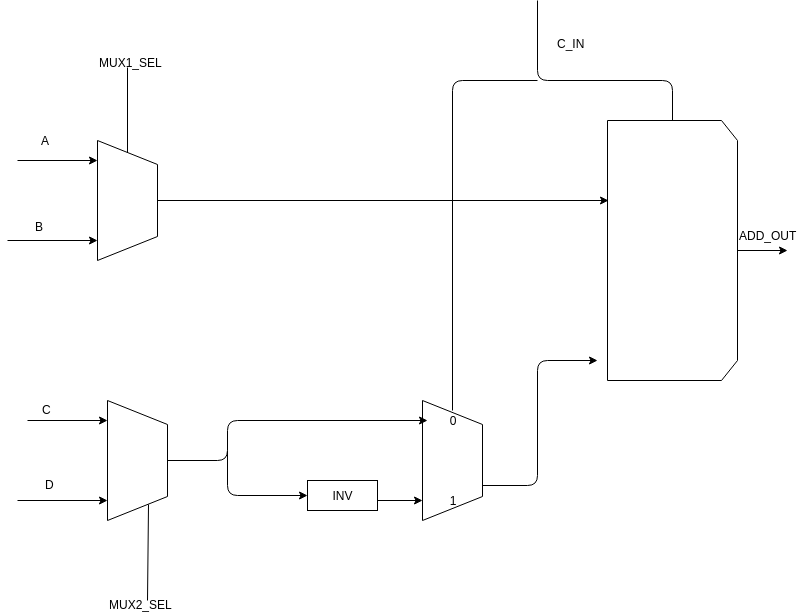
\includegraphics[width=\textwidth]{chapters/figures/adder}
	%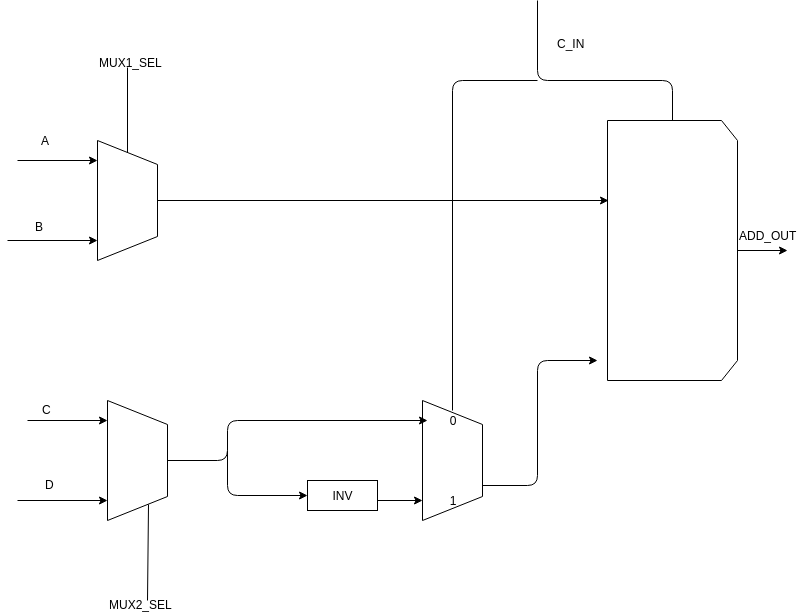
\includegraphics[width=\textwidth]{chapters/figures/adder}
	\caption{Adder with inverter and related selection signal}
	\label{adder_fig}
\end{figure}


\subsection{Logic}

In order to perform some logic bitwise operations, we have reproduced the microarchitecture that has been used for the \textsf{T2}. Here, in figure \ref{logic_fig} is briefly reported the gates needed, that combined between each other, are capable of giving us the desired operations, as reported in the table \ref{logicT2_table}.

\begin{table}[ht]
	\centering
	\begin{tabular}{c|cccc}
		\toprule
				& S0 	& S1	& S2	& S3 \\
		\midrule
		AND		& 0		& 0		& 0		& 1	 \\
		NAND	& 1		& 1		& 1		& 0	 \\
		OR		& 0		& 1		& 1		& 0	 \\
		NOR		& 1		& 0		& 0		& 0	 \\
		XOR		& 0		& 1		& 1		& 0	 \\
		XNOR	& 1		& 0		& 0		& 1	 \\
		\bottomrule
	\end{tabular}
	\caption{Combination of control signal for logic operations}
	\label{logicT2_table} % here is the table label
\end{table}

The control signal \textit{S} is required to be on 4 bits: for this reason, we have implemented in our control word 4 bits for this purpose. In particular, the signal \textsf{OP\_SEL} plays this role. We could have used 3 bits on the \textit{CW} and design an encoder, but the savings in term of connection would have been ruined by the need of an additional decoder. Moreover, these bits are not switched most of the time, thus providing a not so relevant switching power dissipation.

\begin{figure}
	\centering
	%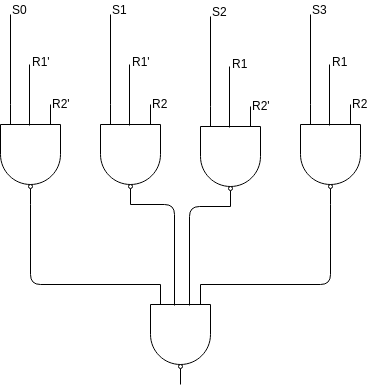
\includegraphics[width=\textwidth]{chapters/figures/logicT2}
	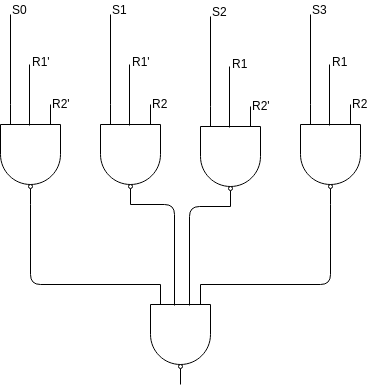
\includegraphics[scale=0.6]{chapters/figures/logicT2}
	\caption{T2 logic for a single bit}
	\label{logic_fig}
\end{figure}

\subsection{Shifter}

To define the lateral shifts, left or right, and the rotation, we have simply provided a behavioral description of the circuit, as reported in appendix \ref{appendix1}. It generates a barrel shifter, thus providing the needed operation between the ones possible, and moving the bits of the first input by the quantity that is introduced by the second input.

\subsection{Logic comparison}

The logic comparison requires the output of the subtraction between the two values to be compared. So, \textit{ADD\_OUT}, output of the adder, is here used as an input. Then, all the bits of the result are \textit{NOR\_reduced}. This allows us to see if all the bits are equal to $0$, i.e. the two operands are equal.
In this case, an additional signal \textit{US} is used, to differentiate between an unsigned or a signed comparison. While in the first case the schematic is the one presented in figure \ref{comp_us_fig}, for the signed case we have to differentiate. As a matter of fact, if the first digit is equal, the two numbers have the same sign, so we can use the same HW presented before. Differently, if the two bits differ, we use what is reported in \ref{comp_s_fig}. The equivalence of the two MSBs is performed through a \textsf{XNOR} gate. 


\begin{figure}
	\centering
	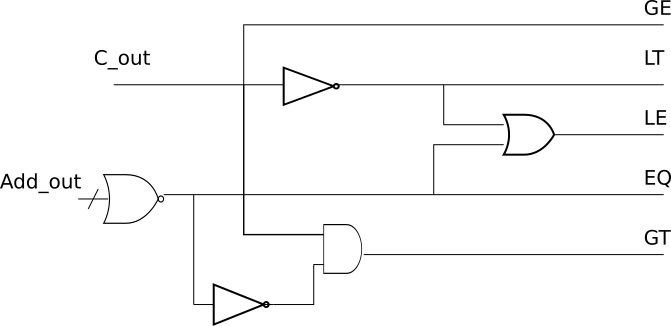
\includegraphics[scale=0.6]{chapters/figures/comp_us}
	\caption{Circuit for comparison - Unsigned}
	\label{comp_us_fig}
\end{figure}


\begin{figure}
	\centering
	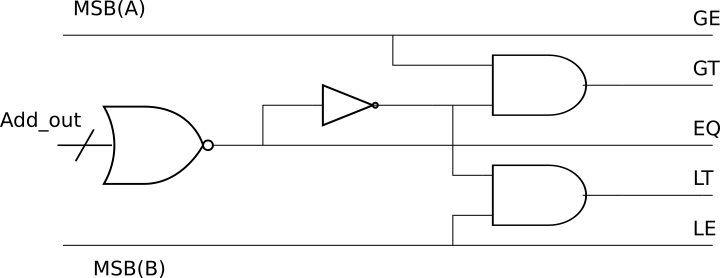
\includegraphics[scale=0.6]{chapters/figures/comp_s1}
	\caption{Comparison for signed case - different MSBs}
	\label{comp_s_fig}
\end{figure}

\begin{figure}
	\centering
	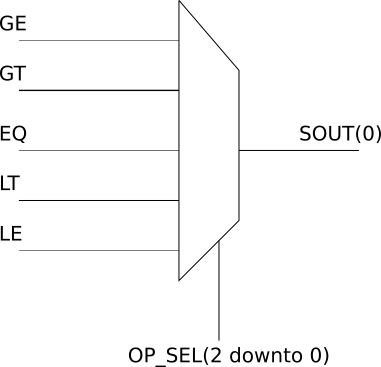
\includegraphics[scale=0.6]{chapters/figures/comp_mux}
	\caption{Mux to select the required condition}
	\label{comp_mux_fig}
\end{figure}


Followingly, the value corresponding to the logic comparison needed is chosen by a mux, whose selection signal is represented by \textit{OP\_SEL}, and assigned to the lowest bit of the output signal \textit{SOUT}, as shown in figure \ref{comp_mux_fig}. All the other bits of this signal are independetly set to $0$.

\subsection{Multiplier}

For our multiplier we again reused the \textit{Booth} architecture that has been designed for the laboratories. As said, the multiplication is usually supposed to be divided in more than one stage, but here it works on a single one, thus reducing the operating frequency. However, we decided to include this component in order to include the MUL in our instruction set. 

\subsection{PC adder}
\noindent
\begin{wrapfigure}{r}{0.4\textwidth}
	\begin{center}
		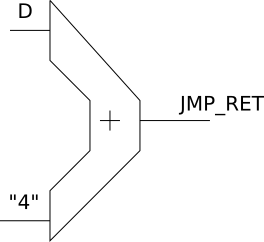
\includegraphics[scale=0.6]{chapters/figures/pc_add}
	\end{center}
	\caption{PC adder}
	\label{pc_add_fig}
\end{wrapfigure}

In order to perform correctly some jump instruction, we need to calculate both 
the new and the return address, which is the PC coming from the previous stage 
+4 and due to the design of our datapath, can not be performed by the single 
adder. An additional adder, reported in figure \ref{pc_add_fig} is in charge of 
this specific operation.






